\subsection{Deniz's Filters}

Deniz's filters focus on fundamental image processing operations implemented through direct pixel-by-pixel matrix iteration. The implemented filters demonstrate concepts such as binary segmentation, stochastic distortion, procedural rendering, and color-space manipulation.

\subsubsection{Original Input Images}

The following images were selected as the common input dataset for evaluating the implemented filters.

\begin{figure}[H]
    \centering

    \begin{subfigure}{0.23\textwidth}
        \centering
        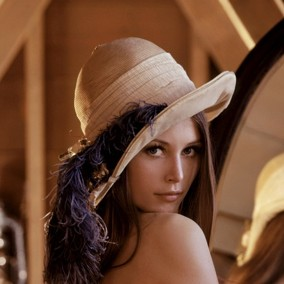
\includegraphics[width=\linewidth]{assets/00.jpg}
        \caption{Input 1}
    \end{subfigure}
    \hfill
    \begin{subfigure}{0.23\textwidth}
        \centering
        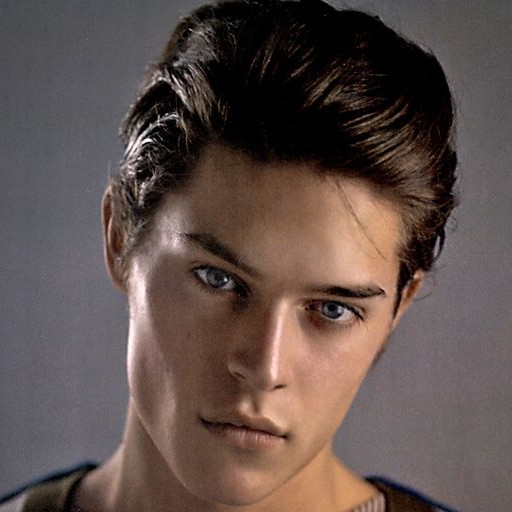
\includegraphics[width=\linewidth]{assets/01.jpg}
        \caption{Input 2}
    \end{subfigure}
    \hfill
    \begin{subfigure}{0.23\textwidth}
        \centering
        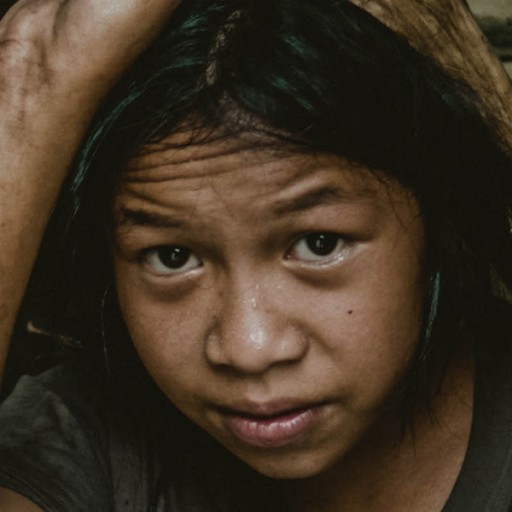
\includegraphics[width=\linewidth]{assets/03.jpg}
        \caption{Input 3}
    \end{subfigure}
    \hfill
    \begin{subfigure}{0.23\textwidth}
        \centering
        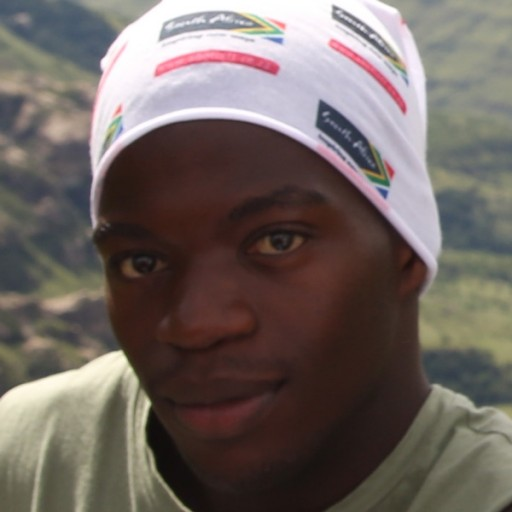
\includegraphics[width=\linewidth]{assets/04.jpg}
        \caption{Input 4}
    \end{subfigure}


@@ -344,14 +344,12 @@ The following images were selected as the common input dataset for evaluating th

\subsubsection{Threshold Filter}

The Threshold filter converts the image into a binary black-and-white representation using grayscale luminosity computation and threshold comparison. It is commonly used in OCR systems, segmentation, and preprocessing pipelines.

\[
L = 0.299R + 0.587G + 0.114B
\]



\[
\text{Output} =
\begin{cases}

@@ -360,18 +358,12 @@ This weighted grayscale formula reflects the sensitivity of the human visual sys
\end{cases}
\]

The algorithm processes each pixel independently with linear complexity:





\[
O(W \times H)
\]



\begin{figure}[H]
    \centering



@@ -399,32 +391,24 @@ where \(W\) and \(H\) represent the width and height of the image respectively.
    \caption{Result 4}
\end{subfigure}

    \caption{Results after applying the Threshold filter.}
    \label{fig:threshold_results}
\end{figure}

\subsubsection{Diffuse Filter}

The Diffuse filter creates a frosted-glass effect by randomly replacing each pixel with a neighboring pixel within a selected radius.



\[
(x', y') = (x + r_x,\ y + r_y)
\]

The filter produces stochastic local distortions while maintaining linear computational complexity:





\[
O(W \times H)
\]



\begin{figure}[H]
    \centering



@@ -452,87 +436,69 @@ although random memory access patterns may slightly reduce cache efficiency comp
    \caption{Result 4}
\end{subfigure}

    \caption{Results after applying the Diffuse filter.}
    \label{fig:diffuse_results}
\end{figure}

\subsubsection{Crosshatch Filter}

The Crosshatch filter simulates sketch-style rendering using procedural diagonal line generation based on pixel coordinates.



\[
(x + y) \bmod n = 0
\]

Darker image regions generate denser hatch patterns, creating a pen-and-ink drawing effect.





\[
O(W \times H)
\]



\begin{figure}[H]
    \centering

    \begin{subfigure}{0.23\textwidth}
        \centering
        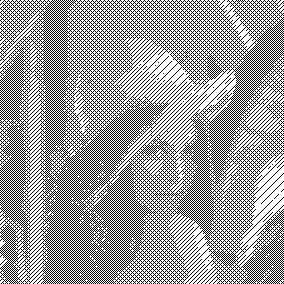
\includegraphics[width=\linewidth]{assets/cross_1.png}
        \caption{Result 1}
    \end{subfigure}
    \hfill
    \begin{subfigure}{0.23\textwidth}
        \centering
        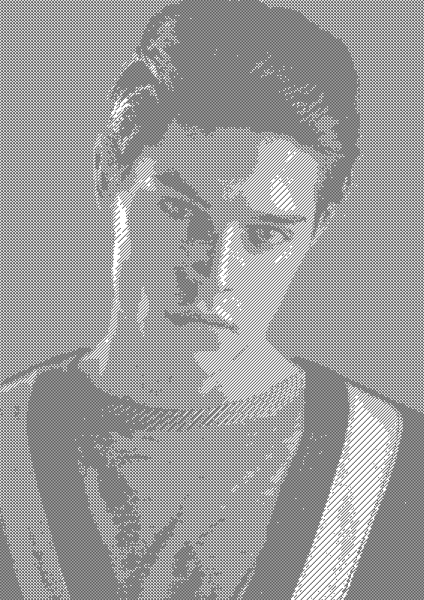
\includegraphics[width=\linewidth]{assets/cross_2.png}
        \caption{Result 2}
    \end{subfigure}
    \hfill
    \begin{subfigure}{0.23\textwidth}
        \centering
        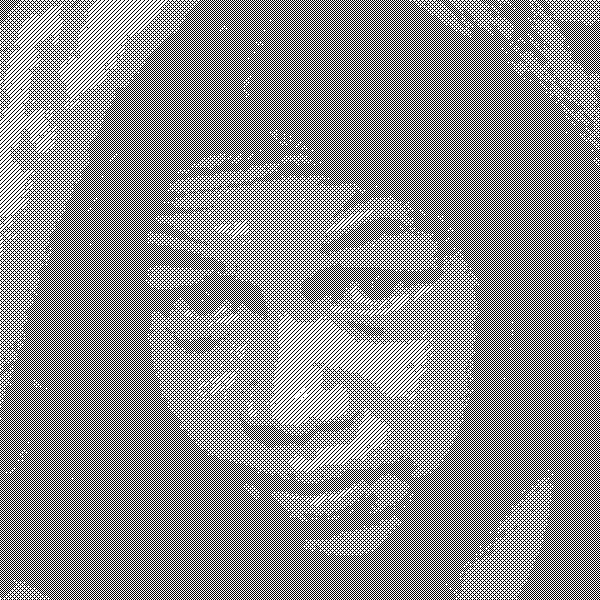
\includegraphics[width=\linewidth]{assets/cross_3.png}
        \caption{Result 3}
    \end{subfigure}
    \hfill
    \begin{subfigure}{0.23\textwidth}
        \centering
        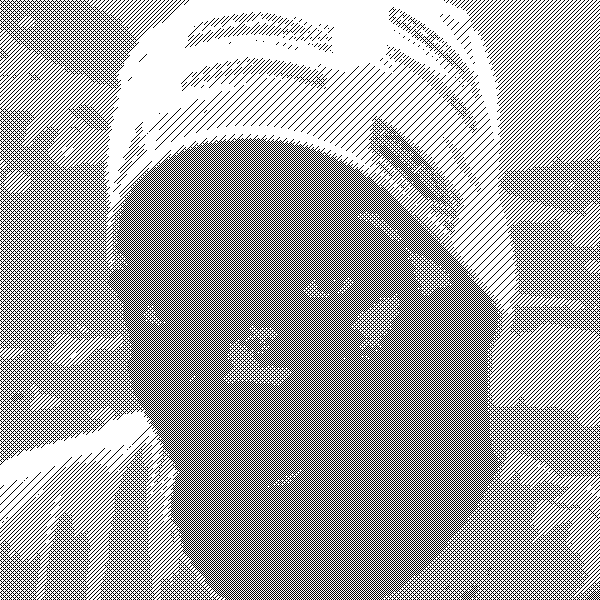
\includegraphics[width=\linewidth]{assets/cross_4.png}
        \caption{Result 4}
    \end{subfigure}

    \caption{Results after applying the Crosshatch filter.}
    \label{fig:crosshatch_results}
\end{figure}

\subsubsection{Hue Rotate Filter}

The Hue Rotate filter modifies image colors by rotating the Hue channel in HSV color space.



\[
H' = (H + \Delta H) \bmod 180
\]

The implemented version applies a \(60^\circ\) hue shift while preserving brightness and structural information.







\[
O(W \times H)
\]



\begin{figure}[H]
    \centering



@@ -560,13 +526,9 @@ since each pixel is processed independently.
    \caption{Result 4}
\end{subfigure}

    \caption{Results after applying the Hue Rotate filter.}
    \label{fig:hue_results}
\end{figure}


